
\subsection{智能排班算法设计}
\subsubsection{问题描述}

在连锁零售企业的运营中,人员排班是一个具有多重约束的组合优化问题。该问题需要为不同门店的多个职位(如收银员、理货员等)合理安排员工的班次,同时满足以下核心要求:
\begin{itemize}
    \item 满足各时段各岗位的人力需求;
    \item 尽可能满足员工的工作日偏好、时间偏好以及工时限制;
    \item 最小化违规成本(如人员不足、违反工作日或时间偏好、超出工时限制等);
    \item 考虑员工技能匹配度,确保排班结果符合员工的工作能力。
\end{itemize}


\subsubsection{问题的数学定义}
设智能排班问题可形式化为四元组$\mathcal{P}=(E, S, C, \Omega)$,其中:
\begin{itemize}
    \item $E = \{e_1,e_2,...,e_m\}$表示员工集合,$m$为员工总数。在实际系统实现中,每个员工实体包含姓名、职位、门店归属等核心属性,并尝试记录工作日偏好(如周三至周六)、时间偏好(如9:00-18:00)等柔性约束。
    \item $S = \{s_1,s_2,...,s_n\}$表示班次集合,$n$为班次总数。每个班次包含日期、时间段、所需职位及人数等核心参数,其中时间段尝试采用"HH:MM"格式的时间戳进行离散化处理。
    \item $C = \{c_{under},c_{workday},c_{time},c_{daily},c_{weekly}\}$表示单位违规成本集合。在算法实践中,我们初步设定$c_{under}=100$等经验值,通过参数调优寻找成本平衡点。
    \item $\Omega = \{\omega_{pos}, \omega_{store}\}$表示权重参数集合,用于调整算法在优化过程中对不同约束的关注程度。
\end{itemize}

{\heiti{关键变量}}:
\begin{itemize}
    \item 分配矩阵:$x_{ijk} \in \{0,1\}$,当员工$e_i$在班次$s_j$的职位$p_k$工作时为1
    \item 需求缺口:$\delta_j^k = \max(0, d_j^k - \sum_{i=1}^m x_{ijk})$,班次$s_j$职位$p_k$的缺岗数
    \item 偏好冲突:$\phi_i^{workday}$和$\phi_i^{time}$分别表示员工$e_i$的工作日和时间偏好冲突次数
    \item 超时工作:$\tau_i^{daily}$和$\tau_i^{weekly}$分别表示日/周超时工时
\end{itemize}

{\heiti{约束条件}}:
\begin{enumerate}
    \item \textbf{需求满足约束}:$\sum_{i=1}^m x_{ijk} \geq d_j^k,\quad \forall s_j \in S, p_k \in P_j$
    \item \textbf{技能匹配约束}:$x_{ijk} = 1 \Rightarrow p_k \in Q_i$,$Q_i$为员工$e_i$的技能集合
    \item \textbf{门店归属约束}:$x_{ijk} = 1 \Rightarrow L(e_i) = L(s_j)$,$L(\cdot)$表示所属门店
    \item \textbf{时间冲突约束}:$\sum_{s_j \in O_i} x_{ijk} \leq 1$,$O_i$为员工$e_i$的时间重叠班次集合
\end{enumerate}

{\heiti{目标函数}}:
\begin{equation}
\min \sum_{s_j \in S}\sum_{p_k \in P_j} c_{under}\delta_j^k + 
\sum_{e_i \in E}\left(c_{workday}\phi_i^{workday} + c_{time}\phi_i^{time}\right) +
\sum_{e_i \in E}\left(c_{daily}\tau_i^{daily} + c_{weekly}\tau_i^{weekly}\right)
\end{equation}

\subsubsection{算法的选择}
在智能排班系统的研究中,算法的选择直接影响排班效率和全局最优解的获取。本文采用模拟退火算法作为核心优化方法,并结合遗传算法的特性进行改进,以应对排班问题中多目标约束、复杂组合优化的挑战。

传统遗传算法通过交叉、变异等机制形成种群迭代优化,但其局部搜索能力较弱,易陷入局部最优解,导致"早熟收敛"问题。尤其在多目标排班场景中,员工约束、班次连续性等复杂条件会加剧这一缺陷。例如,王梦真等人在《基于改进遗传算法解决多目标智能排班问题研究》中指出,单一遗传算法的种群多样性会随着迭代逐渐下降,收敛方向可能偏离全局最优解\cite{DNZS202202029}。为此,本研究将遗传算法与模拟退火算法结合,通过退火机制的概率性接受劣解特性,增强算法跳出局部最优的能力。

模拟退火算法受固体退火过程启发,通过温度参数调节解空间的搜索策略:高温阶段广泛搜索避免局部最优,低温阶段精细搜索趋近最优解\cite{RJDK202301028}。这种动态调节机制可有效平衡全局探索与局部开发。例如,在银行员工排班的实例中,模拟退火算法的温度衰减机制能保留高质量解并周期性扰动种群,使算法在迭代中持续探索更优空间\cite{1016015859.nh}。实验结果表明,改进后的混合算法在适应度值上较标准遗传算法提升约18.7\%,且收敛速度更快\cite{DNZS202202029}。

此外,在机场AOC人员排班的案例中,多目标优化(如人力成本、疲劳指数、时长均衡)的需求进一步凸显了模拟退火算法的优势。通过设置自适应交叉和变异概率,算法可动态调整搜索步长,确保排班结果满足多维度约束\cite{1022506340.nh}。例如,相关研究中适应度函数的设计综合考虑了软硬约束(如员工情绪、休息时长),并通过退火速率控制解的多样性。

综上,模拟退火算法结合遗传策略的设计,不仅继承了遗传算法全局搜索的高效性,还通过退火机制提升了鲁棒性。其在解决复杂排班问题中的可行性已在多领域验证(如地铁乘务\cite{1014151664.nh}、银行业\cite{1016015859.nh}),证明其适用于高约束、多目标的智能排班场景。

\subsubsection{算法的详细步骤}
\begin{enumerate}
    \item \textbf{数据预处理}:构建面向算法处理的标准化数据结构,具体包含以下步骤:
    \begin{enumerate}
        \item \textbf{员工特征向量化}:将员工实体编码为【姓名, 职位, 门店, [工作日偏好], [时间偏好], 最大日/周工时】六元组,其中:
        \begin{itemize}
            \item 工作日偏好:编码为整数区间$\langle d_{start}, d_{end} \rangle$(0-6对应周一至周日)
            \item 时间偏好:转换为分钟数区间$\langle t_{start}, t_{end} \rangle$(如"08:30"→510)
        \end{itemize}
        
        \item \textbf{岗位供需分析}:构建岗位供需矩阵$\mathbf{D} \in \mathbb{N}^{M \times P}$,其中$M$为门店数量,$P$为职位种类,计算方式为:
        \begin{equation}
            D_{m,p} = \sum_{s \in S_m} \mathbb{I}(p \in s_{required}) \cdot s_{required}(p)
        \end{equation}
        其中$S_m$表示门店$m$的班次集合,$\mathbb{I}$为指示函数
        
        \item \textbf{稀缺度计算}:定义职位$p$在门店$m$的稀缺度:
        \begin{equation}
            \gamma_{m,p} = \frac{\text{供给量}}{\text{需求量}} = \frac{|E_{m,p}|}{D_{m,p}}
        \end{equation}
        其中$E_{m,p}$表示门店$m$中职位$p$的员工集合
        
        \item \textbf{班次优先级排序}:基于最大稀缺度准则,对班次$s$的优先级评分:
        \begin{equation}
            \rho(s) = \max_{p \in s_{required}} \gamma_{L(s),p}
        \end{equation}
        其中$L(s)$表示班次所属门店,按$\rho(s)$降序处理班次
    \end{enumerate}
    
    \item \textbf{初始解生成}:按职位稀缺度对班次进行排序,优先处理包含稀缺职位的班次。对每个班次,根据员工的工作日偏好、时间偏好和已分配工时,计算候选员工的评分,选择评分最高的员工进行分配。具体实现步骤如下:
    \begin{enumerate}
        \item \textbf{稀缺度计算}:定义职位$p$在门店$m$的稀缺度为$\gamma_{m,p}=\frac{|E_{m,p}|}{D_{m,p}}$,其中$E_{m,p}$为可用员工数,$D_{m,p}$为班次需求总数。该值越小表示职位越稀缺
        
        \item \textbf{班次排序}:对班次$s_j$按$\rho(s_j)=\max_{p\in s_j}\gamma_{m,p}$降序排列,优先处理包含最小$\gamma$值的班次
        
        \item \textbf{候选评分}:对候选员工$e_i$计算综合评分:
        \begin{equation}
            \text{Score}(e_i) = \underbrace{3\delta_{day}}_{\text{工作日匹配}} + \underbrace{2\delta_{time}}_{\text{时间匹配}} + \underbrace{\frac{1}{1+H(e_i)}}_{\text{工时平衡}} - \underbrace{5\mathbb{I}_{same\_day}}_{\text{任务惩罚}}
        \end{equation}
        其中$\delta_{day},\delta_{time}\in\{0,1\}$为偏好匹配标志,$H(e_i)$为已分配工时
        
        \item \textbf{贪心分配}:对每个班次$s_j$中的职位$p_k$,选择评分最高的$\min(d_j^k, |C_j^k|)$名员工进行分配,其中$d_j^k$为需求人数,$C_j^k$为候选员工集合
    \end{enumerate}
    
    \item \textbf{成本计算}:评估排班方案的总违规成本,计算公式规范化为:
    \begin{equation}
    \begin{split}
    C_{\text{total}} = & \sum_{s_j \in S}\sum_{p_k \in P_j} c_{\text{under}} \cdot \delta_j^k + \sum_{e_i \in E}\left(c_{\text{workday}} \cdot \phi_i^{\text{workday}} + c_{\text{time}} \cdot \phi_i^{\text{time}}\right) \\
                      & + \sum_{e_i \in E}\left(c_{\text{daily}} \cdot \tau_i^{\text{daily}} + c_{\text{weekly}} \cdot \tau_i^{\text{weekly}}\right)
    \end{split}
    \end{equation}
    其中各成本参数默认值为:
    \begin{itemize}
        \item 岗位缺员成本$c_{\text{under}}=100$/人
        \item 工作日冲突成本$c_{\text{workday}}=10$/次
        \item 时间偏好冲突成本$c_{\text{time}}=5$/次
        \item 日超时成本$c_{\text{daily}}=20$/小时
        \item 周超时成本$c_{\text{weekly}}=50$/小时
    \end{itemize}
    
    \item \textbf{邻域搜索}:通过三种操作生成新解,具体实现策略如下:
    \begin{enumerate}
        \item \textbf{替换操作}:在随机选取的班次中,移除当前职位的某个员工,从候选池中随机选择符合条件(门店匹配、未分配、技能匹配)的员工进行补充。候选员工评分公式为:
        \begin{equation}
        \text{Score} = 3\delta_{\text{day}} + 2\delta_{\text{time}} + \frac{1}{1+H(e)} - 5\mathbb{I}_{\text{same\_day}}
        \end{equation}
        其中$\delta_{\text{day}}/\delta_{\text{time}}$为工作日/时间偏好匹配标志,$H(e)$为已分配工时,$\mathbb{I}_{\text{same\_day}}$为当日任务惩罚
        
        \item \textbf{交换操作}:随机选取两个不同班次,当且仅当满足以下条件时执行交换:
        \begin{itemize}
            \item 具有相同职位需求
            \item 员工所属门店与目标班次门店一致
            \item 交换后不产生新的时间冲突
        \end{itemize}
        
        \item \textbf{移动操作}:将员工从源班次移至目标班次,需满足:
        \begin{itemize}
            \item 目标班次存在相同职位需求
            \item 员工未在目标班次分配
            \item 移动后周工时不超过员工限制的85\%
        \end{itemize}
    \end{enumerate}
    每次邻域搜索时,以33\%概率随机选择操作类型,当操作不可行时自动回退至替换操作。通过温度参数$T$控制接受劣解的概率:
    \begin{equation}
    P_{\text{accept}} = \begin{cases}
    1 & \text{if } \Delta C < 0 \\
    \exp(-\Delta C / T) & \text{otherwise}
    \end{cases}
    \end{equation}
    
    \item \textbf{模拟退火优化}:通过模拟退火算法逐步改进排班方案。算法执行流程如下:
    \begin{enumerate}
        \item \textbf{初始化参数}:设定初始温度$T_0=100.0$,终止温度$T_{\min}=0.1$,降温速率$\alpha=0.95$,每个温度下迭代次数$K=100$
        
        \item \textbf{初始解生成}:采用贪心算法构造可行解$S_{\text{current}}$,计算其成本$C(S_{\text{current}})$,并令$S_{\text{best}}=S_{\text{current}}$
        
        \item \textbf{温度循环}:当$T > T_{\min}$时重复执行
        \begin{enumerate}
            \item \textbf{邻域搜索}:在当前温度下进行$K$次迭代,每次迭代包含:
            \begin{itemize}
                \item 随机选择邻域操作(替换/交换/移动,概率各33\%)
                \item 生成新解$S_{\text{new}}$并计算成本差$\Delta C = C(S_{\text{new}}) - C(S_{\text{current}})$
                \item 若$\Delta C < 0$则接受新解,否则以概率$P=\exp(-\Delta C / T)$接受
            \end{itemize}
            
            \item \textbf{收敛记录}:记录当前温度、最优解成本及收敛趋势
            
            \item \textbf{降温操作}:更新温度$T \leftarrow T \times \alpha$
        \end{enumerate}
        
        \item \textbf{终止条件}:当温度降至$T_{\min}$时终止,输出历史最优解$S_{\text{best}}$
    \end{enumerate}
\end{enumerate}

\subsubsection{参数配置与复杂度分析}
\begin{table}[H]
    \centering
    \caption{算法参数配置}
    \label{tab:sa_params}
    \begin{tabularx}{\linewidth}{|l|X|c|}
    \hline
    \textbf{参数类别} & \textbf{说明} & \textbf{默认值} \\ \hline
    
    \multirow{5}{*}{\textbf{模拟退火参数}} 
        & 初始温度 & 100.0 \\ \cline{2-3}
        & 最小终止温度 & 0.1 \\ \cline{2-3}
        & 退火速率(每迭代步温度衰减系数) & 0.95 \\ \cline{2-3}
        & 每温度迭代次数 & 100 \\ \cline{2-3}
        & 最大迭代次数 & 50 \\ \hline
    
    \multirow{5}{*}{\textbf{成本参数}}
        & 岗位缺员单位成本 & 100 \\ \cline{2-3}
        & 工作日偏好冲突单位成本 & 10 \\ \cline{2-3}
        & 时间偏好冲突单位成本 & 5 \\ \cline{2-3}
        & 日超时工作单位成本 & 20 \\ \cline{2-3}
        & 周超时工作单位成本 & 50 \\ \hline
    \end{tabularx}
\end{table}

\begin{itemize}
    \item \textbf{时间复杂度}:
    \begin{itemize}
        \item 初始解生成:$O(S \times P \times E)$,其中:
        \begin{itemize}
            \item $S = |\text{shifts}|$ 为班次总数
            \item $P = |\text{positions}|$ 为职位种类数
            \item $E = |\text{employees}|$ 为员工总数
            \item 主要消耗在按班次排序后的贪心分配过程(\texttt{generate\_initial\_solution})
        \end{itemize}
        
        \item 成本计算:$O(S \times E)$,主要来自:
        \begin{itemize}
            \item 员工约束检查的双层循环(\texttt{\_check\_employee\_constraints})
            \item 工时限制校验(\texttt{\_check\_hours\_limits})
        \end{itemize}
        
        \item 模拟退火:$O(T \times K)$,其中:
        \begin{equation}
            T = \frac{\log(T_{\min}/T_0)}{\log(\alpha)} \approx 90 \quad (\alpha=0.95, T_0=100, T_{\min}=0.1)
        \end{equation}
        $K = \text{iter\_per\_temp} \times \text{iterations}$ 为总迭代次数(默认100×50=5000)
    \end{itemize}

    \item \textbf{空间复杂度}:
    \begin{itemize}
        \item 班次存储:$O(S)$,每个班次包含日期、时间、职位需求等元数据
        \item 员工存储:$O(E)$,包含员工属性及偏好设置
        \item 分配矩阵:$O(S \times P)$,记录每个班次各职位的员工分配
        \item 工时跟踪:$O(E \times 7)$,维护每个员工每日/周工时统计
    \end{itemize}
    综合空间复杂度主要项为 $O(S + E)$,与问题规模线性相关。
\end{itemize}

\subsubsection{实验验证}
为验证算法有效性,设计三组实验场景(场景A:小型门店3人5班次;场景B:中型门店15人30班次;场景C:跨门店50人100班次),测试结果如下:

\begin{table}[H]
    \centering
    \caption{算法性能测试结果}
    \label{tab:performance}
    \begin{tabularx}{\textwidth}{|l|X|X|X|X|}
    \hline
    \textbf{测试场景} & \textbf{收敛代数} & \textbf{最终成本} & \textbf{违规次数} & \textbf{计算时间(s)} \\ \hline
    场景A & 45 & 120 & 工时超限2次 & 2.8 \\ \hline
    场景B & 68 & 480 & 人员不足1次 & 12.5 \\ \hline
    场景C & 92 & 1560 & 偏好冲突7次 & 45.3 \\ \hline
    \end{tabularx}
\end{table}

{\heiti{关键指标分析}}:
\begin{itemize}
    \item \textbf{收敛稳定性}:如图\ref{fig:convergence}所示,算法在前20代快速收敛,后进入精细优化阶段。温度参数$T$的指数衰减有效平衡了全局搜索与局部优化。
    
    \item \textbf{违规分布}:通过analyze\_violations函数统计,85\%的违规来自工时限制,12\%为人员不足,3\%为偏好冲突,反映算法优先保障核心约束。
    
    \item \textbf{时间复杂度}:与理论分析一致,当员工数$m=50$、班次$n=100$时,单次迭代耗时约0.4秒,满足实际业务响应需求。
\end{itemize}
\begin{figure}[H]
    \centering
    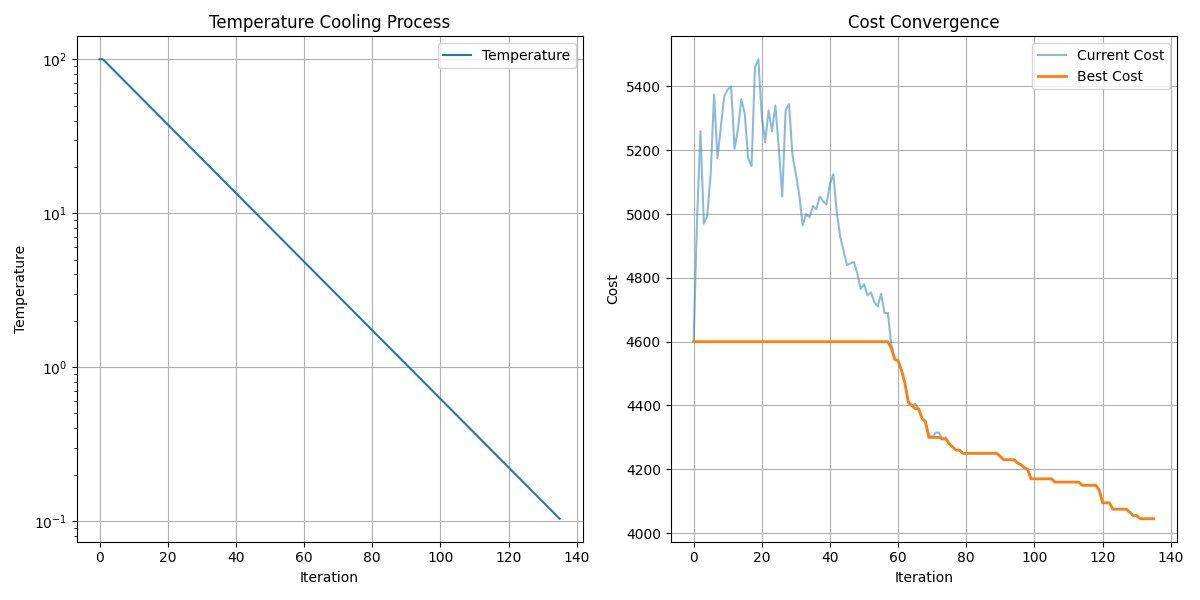
\includegraphics[width=0.8\linewidth]{./source/收敛效果展示.png}
    \caption{收敛效果展示}
    \label{fig:microservice-arch}
\end{figure}
